\documentclass[10pt, twoside, a4paper]{article}
\usepackage{graphicx}
\usepackage{listings}
  
\title{marca - McAdam's RISC Computer Architecture\\Implementation Details}
\author{Wolfgang Puffitsch}

\begin{document}

  \maketitle

  \section{General}
  
  \begin{itemize}
  \item 16 16-bit registers
  \item 16KB instruction ROM (8192 instructions)
  \item 8KB data RAM
  \item 256 byte data ROM
  \item 75 instructions
  \item 16 interrupt vectors
  \end{itemize}

  \section{Internals}

  The processor features a 4-stage pipeline:
  \begin{itemize}
  \item instruction fetch
  \item instruction decode
  \item execution/memory access
  \item write back
  \end{itemize}
  This scheme is similar to the one used in the MIPS architecture,
  only execution and write back stage are drawn together. For our
  architecture does not support indexed addressing, it does not need
  the ALU's result and can work in parallel, having the advantage of
  reducing the possible hazards.

  Figure \ref{fig:marca} shows a rough scheme of the internals of the
  processor.
  \begin{figure}[ht!]
    \centering
    \includegraphics[width=.95\textwidth]{marca}
    \caption{Internal scheme}
    \label{fig:marca}
  \end{figure}

  \subsection{Branches}
  Branches are not predicted and if executed they stall the the
  pipeline, leading to a total execution time of 4 cycles. The fetch
  stage is not stalled, the decode stage however is stalled for two
  cycles to compensate that.

  \subsection{Instruction fetch}
  This stage is not spectacular: it simply reads an instruction from
  the instruction ROM, and extracts the bits for the source and
  destination registers.

  \subsection{Instruction decode}
  This stage translates the bit-patterns of the opcodes to the signals
  used internally for the operations. It also holds the register file
  and handles access to it. Immediate values are also constructed here.

  \subsection{Execution / Memory access}
  The execution stage is the heart and soul of the processor: it holds
  the ALU, the memory/IO unit and a unit for interrupt handling.

  \subsubsection{ALU}
  The ALU does all arithmetic and logic computations as well as taking
  care of the processors flags (which are organized as seen in table
  \ref{tab:flags}).

  \begin{table}[ht!]
    \centering
    \begin{tabular}{|p{.75em}|p{.75em}|p{.75em}|p{.75em}
                    |p{.75em}|p{.75em}|p{.75em}|p{.75em}
		    |p{.75em}|p{.75em}|p{.75em}|p{.75em}
		    |p{.75em}|p{.75em}|p{.75em}|p{.75em}|p{.75em}}
      \multicolumn{16}{c}{Bit 15 \hfill Bit 0} \\
      \hline
      & & & & & & & & & & P & I & N & V & C & Z \\
      \hline
    \end{tabular}
    \caption{The flag register}
    \label{tab:flags}
  \end{table}

  Operations which need more than one cycle to execute (multiplication,
  division and modulo) block the rest of the processor until they are
  finished.

  \subsubsection{Memory/IO unit}
  The memory/IO unit takes care of the ordinary data memory, the data
  ROM (which is mapped to the addresses right above the RAM) and the
  communication to peripheral modules. Peripheral modules are located
  within the memory/IO unit and mapped to the highest addresses.

  The memories (the instruction ROM too) are Altera specific; we
  decided not to use generic memories, because \textsl{Quartus} can update the
  contents of its proprietary ROMs without synthesizing the whole
  design. Because all memories are single-ported (and thus fairly
  simple) it should be easy to replace them with memories specific to
  other vendors.

  We also decided against the use of external memories; larger FPGAs
  can accommodate all addressable memory on-chip, so the implementation
  overhead would not have paid off.

  Accesses which take more than one cycle (stores to peripheral
  modules and all load operations) block the rest of the processor
  until they are finished.

  \paragraph{Peripheral modules}
  The peripheral modules use a slightly modified version of the SimpCon
  interface. The SimpCon specific signals are pulled together to
  records, and the words which can be read/written are limited to 16
  bits. For accessing such a module, one may only use \texttt{load}
  and \texttt{store} instructions which point to aligned addresses.

  \paragraph{UART}
  The built-in UART is derived from the sc\_uart from Martin
  Sch\"oberl.  Apart from adapting the SimpCon interface, an interrupt
  line and two bits for enabling/masking receive (bit 3 in the status
  register) and transmit (bit 2) interrupts. In the current version
  address 0xFFF8 (-8) correspond to the UART's status register and
  address 0xFFFA (-6) to the wr\_data/rd\_data register.

  \subsubsection{Interrupt unit}
  The interrupt unit takes care of the interrupt vectors and, of
  course, the triggering of interrupts. Interrupts are executed only
  if the global interrupt flag is set, none of the other units is busy
  and the instruction in the execution stage is valid (it takes 3
  cycles after jumps, branches etc. until a new valid instruction is
  in that stage).

  Instructions which cannot be decoded as well as the ``error''
  instruction trigger interrupt 0; the ALU can trigger interrupt 1
  (division by zero), the memory unit can trigger interrupt 2 (invalid
  memory access). In contrast to all other interrupts, these three
  interrupts do not repeat the instruction which is executed when they
  occur.

  \subsection{Write back}
  The write back stage passes on the result of the execution stage to
  all other stages.

  \section{Assembler}
  The assembler \textsl{spar} (SPear Assembler Recycled) uses a syntax
  quite like usual Unix-style assemblers. It accepts the pseudo-ops
  \texttt{.file}, \texttt{.text}, \texttt{.data}, \texttt{.bss},
  \texttt{.align}, \texttt{.comm}, \texttt{.lcomm}, \texttt{.org} and
  \texttt{.skip} with the usual meanings. The mnemonic \texttt{data}
  initializes a byte to some constant value. In difference to the
  instruction set architecture specification, \texttt{mod} and
  \texttt{umod} accept three operands (if a move is needed, it is
  silently inserted).

  The assembler produces three files: one file for the instruction
  ROM, one file for the even bytes of the data ROM and one file for
  the odd bytes of the instruction ROM. The splitting of the data is
  necessary, because the data memories internally are split into two
  8-bit memories in order to support unaligned memory accesses without
  delays.

  Three output formats are supported: .mif (Memory Initialization
  Format), .hex (Intel Hex Format) and a binary format designed for
  download via UART.

  \section{Resource usage and speed}

  The processor was synthesized with \textsl{Quartus II} for the
  \textsl{Cyclone EP1C12Q240C8} FPGA with 12060 logic cells and 29952
  bytes of on-chip memory available.

  The processor needs $\sim$3550 logic cells or 29\% when being
  compiled for maximum clock frequency, which is $\sim$60 MHz. When
  optimizing for area, it needs $\sim$2600 logic cells or 22\% at
  $\sim$25 MHz.

  The processor uses 24832 bytes or 83\% of on-chip memory.

  \section{Example}

  \subsection{Reversing a line}

  In listing \ref{lst:uart} one can see how to interface the uart via
  interrupts. The program reads in a line from the UART and the writes
  it back reversed. The lines 1 to 4 show how to instantiate memory
  (the two bytes defined form the DOS-style end-of-line). The
  lines 7 to 25 initialize the registers and register the interrupt
  vectors, line 28 builds a barrier against the rest of the code.

  The lines 32 to 76 form the interrupt service routine. It first
  checks if it is operating in read or in write mode. When reading, it
  reads from the UART and stores the result. A mode switch occurs when
  a newline character is encountered. In write mode the contents of
  the buffer is written to the UART and switching back to read mode is
  done when finished.

  In figure \ref{fig:sim} the results of the simulation are presented.

  \lstset{basicstyle=\footnotesize,numbers=left,numberstyle=\tiny}
  \lstset{caption=Example for the UART and interrupts}
  \lstset{label=lst:uart}
  \lstinputlisting{uart_reverse.s}

  \begin{figure}[ht!]
    \centering
    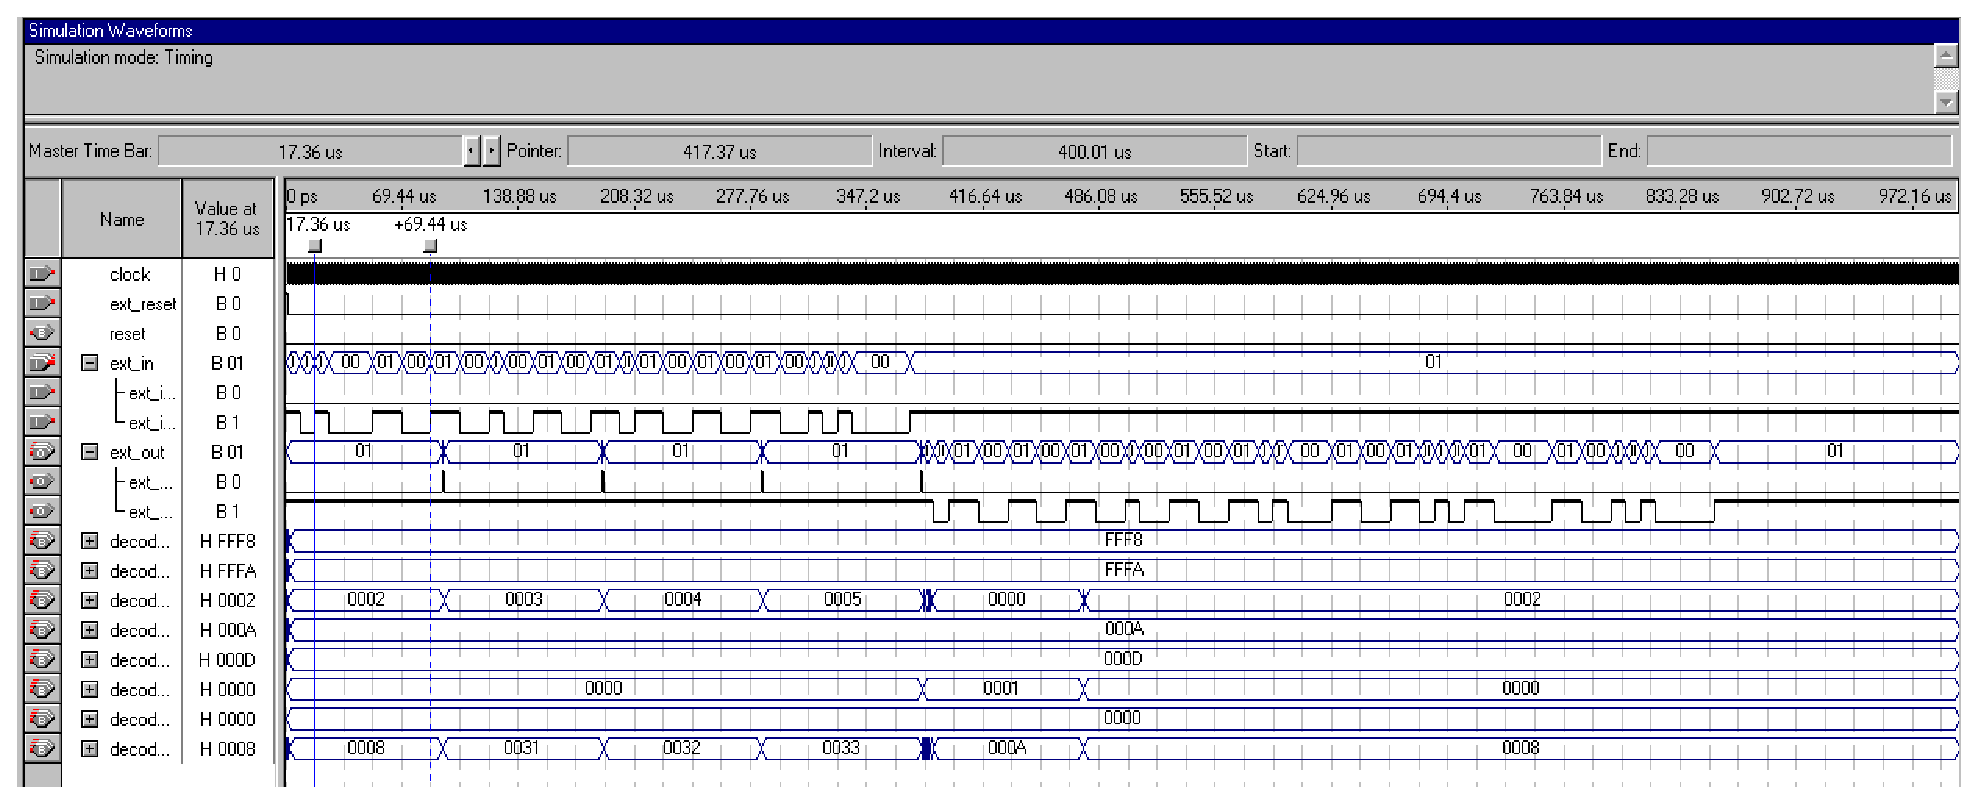
\includegraphics[width=.95\textwidth]{uart_sim}
    \caption{Simulation results}
    \label{fig:sim}    
  \end{figure}

  \subsection{Computing factorials}

  The example in \ref{lst:fact} computes the factorials of 1 \ldots 9
  and writes the results to the PC via UART. Note that the last result
  transmitted will be wrong, because it is truncated to 16 bits.

  \lstset{basicstyle=\footnotesize,numbers=left,numberstyle=\tiny}
  \lstset{caption=Computing factorials}
  \lstset{label=lst:fact}
  \lstinputlisting{factorial.s}
  

  \section{Versions Of This Document}
  
  2006-12-14: Draft version \textbf{0.1}

  \noindent
  2006-12-29: Draft version \textbf{0.2}
  \begin{itemize}
    \item A few refinements.
  \end{itemize}

  \noindent
  2007-01-22: Draft version \textbf{0.3}
  \begin{itemize}
    \item Added another example.
  \end{itemize}

  \noindent
  2007-02-02: Draft version \textbf{0.4}
  \begin{itemize}
    \item Updated resource usage and speed section.
  \end{itemize}

\end{document}
